%=======================================
% ============== PREAMBLE ============== 
% ======================================

% Beamer Presentation
\documentclass[12pt]{beamer}

% Packages
\usepackage[utf8]{inputenc}
\usepackage[T1]{fontenc}
\usepackage{fontspec}
\usepackage[american]{babel}
\usepackage[autostyle]{csquotes}
\usepackage{graphicx}   % Enable PNG,JPEG import
\usepackage{amsthm}     % Theorems
\usepackage{amsfonts}   % AMS fonts
\usepackage{amsmath}    % AMS math
\usepackage{bm}         % For bold font
\usepackage{alltt}      % Easy verbose environment
\usepackage{fixltx2e}   % Fixes
\usepackage{booktabs}   % Proper tables
\usepackage{microtype}

% Beamer (LaTeX PDF presentation) stuff
\usetheme{uleiden}
\beamertemplatenavigationsymbolsempty
\setbeamercolor{alerted text}{fg=uleiden}
\setbeamerfont{footnote}{size=\scriptsize}

\frenchspacing  % Only one space after period

% Bibliography
%\usepackage{biblatex}
\addtobeamertemplate{footnote}{\vspace{-6pt}\advance\hsize-0.5cm}{\vspace{6pt}}
\makeatletter
% Alternative A: footnote rule
\renewcommand*{\footnoterule}{\kern -3pt \hrule \@width 2in \kern 8.6pt}
% Alternative B: no footnote rule
% \renewcommand*{\footnoterule}{\kern 6pt}
\makeatother
\usepackage[style=verbose,autocite=footnote]{biblatex}
% Bibliography
%\bibliographystyle{plainnat}
\bibliography{mybib}

\newtheoremstyle{break}% name
  {}%         Space above, empty = `usual value'
  {}%         Space below
  {\normalfont}% Body font
  {}%         Indent amount (empty = no indent, \parindent = para indent)
  {\bfseries}% Thm head font
  {.}%        Punctuation after thm head
  {\newline}% Space after thm head: \newline = linebreak
  {}%         Thm head spec

\theoremstyle{break}
\newtheorem{mydef}{Definition}  % Environment for definitions

% Bibliography and citation
%\addbibresource{/home/benny/Dropbox/seminar/Paper/V3/pagerank_paper.bib}
%\DeclareFieldFormat[inbook,article]{citetitle}{#1}
%\DeclareFieldFormat[inbook,article]{title}{#1}

% Title page
\title{Entity Resolution in Unstructured Data}
\subtitle{and applications in the analysis of historical documents}
\author{Benjamin van der Burgh}
\date{March 15th 2016}


%%% Separation between items in list
\usepackage{etoolbox}% http://ctan.org/pkg/etoolbox

\makeatletter
\patchcmd{\@listI}{\itemsep3\p@}{\itemsep.7em}{}{}
\makeatother


\makeatletter
\newenvironment{customlist}[2]{
  \ifnum\@itemdepth >2\relax\@toodeep\else
      \advance\@itemdepth\@ne%
      \beamer@computepref\@itemdepth%
      \usebeamerfont{itemize/enumerate \beameritemnestingprefix body}%
      \usebeamercolor[fg]{itemize/enumerate \beameritemnestingprefix body}%
      \usebeamertemplate{itemize/enumerate \beameritemnestingprefix body begin}%
      \begin{list}
        {
            \usebeamertemplate{itemize \beameritemnestingprefix item}
        }
        { \leftmargin=#1 \itemindent=#2
            \def\makelabel##1{%
              {%  
                  \hss\llap{{%
                    \usebeamerfont*{itemize \beameritemnestingprefix item}%
                        \usebeamercolor[fg]{itemize \beameritemnestingprefix item}##1}}%
              }%  
            }%  
        }
  \fi
}
{
  \end{list}
  \usebeamertemplate{itemize/enumerate \beameritemnestingprefix body end}%
}
\makeatother



%%% Packages used for nice quoting
\usepackage{etoolbox}
%\usepackage[svgnames]{xcolor}
\usepackage{tikz}
%\usepackage{framed}
\usepackage{libertine} % or any other font package
\newcommand*\quotefont{\fontfamily{LinuxLibertineT-LF}}

%%% Commands used in nice quoting
\newcommand*\quotesize{40}

\newcommand*{\openquote}
   {\tikz[remember picture,overlay,xshift=-4ex,yshift=-2.5ex]
   \node (OQ) {\quotefont\fontsize{\quotesize}{\quotesize}\selectfont``};\kern0pt}

\newcommand*{\closequote}[1]
  {\tikz[remember picture,overlay,xshift=4ex,yshift={#1}]
   \node (CQ) {\quotefont\fontsize{\quotesize}{\quotesize}\selectfont''};}

% select a colour for the shading
\colorlet{shadecolor}{red}

\newcommand*\shadedauthorformat{\emph}

\newcommand*\authoralign[1]{%
  \if#1l
    \def\authorfill{}\def\quotefill{\hfill}
  \else
    \if#1r
      \def\authorfill{\hfill}\def\quotefill{}
    \else
      \if#1c
        \gdef\authorfill{\hfill}\def\quotefill{\hfill}
      \else\typeout{Invalid option}
      \fi
    \fi
  \fi}

\newenvironment{shadequote}[2][l]%
{\authoralign{#1}
\ifblank{#2}
   {\def\shadequoteauthor{}\def\yshift{-2ex}\def\quotefill{\hfill}}
   {\def\shadequoteauthor{\par\authorfill\shadedauthorformat{#2}}\def\yshift{2ex}}
\begin{quote}\openquote}
{\shadequoteauthor\quotefill\closequote{\yshift}\end{quote}}

%\newcommand\mathmacro[1][A]{\ensuremath{{#1}_1}}
\newcommand*{\parsevar}[1]{\ensuremath{\left\{\textrm{#1}\right\}}}

%%% Colored box around text
\newcommand{\cfbox}[2]{%
    \colorlet{currentcolor}{.}%
    {\color{#1}%
    \fbox{\color{currentcolor}#2}}%
}

%%% Algorithms
\usepackage[noend]{algpseudocode}
\usepackage{algorithm}
\newcommand*\Let[2]{\State #1 $\gets$ #2}                           % Defined for convenience
\newcommand*{\LineFor}[2]{%
    \State\algorithmicfor\ {#1}\ \algorithmicdo\ {#2} \algorithmicend\ \algorithmicfor%
}
\newcommand*{\To}{\:\bm{ to }\:}
\newcommand*{\SizeOf}[1]{\:\vert {#1} \vert\:}


%%% Syntax highlighting in code
\usepackage[cache=false,outputdir=.texpadtmp]{minted}
\usemintedstyle{autumn}
\usepackage{listings}
\definecolor{codebg}{RGB}{248,248,248}

\usepackage{etoolbox}
\AtBeginEnvironment{minted}{\singlespacing%
    \fontsize{10}{10}\selectfont}
    
    
\usepackage{tikz}
\usepackage{pgfplots}
\usepackage{pgfplotstable}
\usepackage{tikzscale}            % Nice scaling of plots
\definecolor{sns1}{HTML}{4c72b0}  % Colors as defined in the 'seaborn' Python package
\definecolor{sns2}{HTML}{55a868}
\definecolor{sns3}{HTML}{c44e52}
\definecolor{sns4}{HTML}{8172b2}
\definecolor{sns5}{HTML}{ccb974}
\definecolor{sns6}{HTML}{64b5cd}
\pgfplotscreateplotcyclelist{seaborn}{
    sns1!70!black, every mark/.append style={solid,fill=sns1},mark=*\\%
    sns2!70!black, every mark/.append style={solid,fill=sns2},mark=square*\\%
    sns3!70!black, every mark/.append style={solid,fill=sns3},mark=triangle*\\%
    sns4!70!black, every mark/.append style={solid,fill=sns4},mark=diamond*\\%
    sns5!70!black, every mark/.append style={solid,fill=sns5},mark=pentagon*\\%
    sns6!70!black, every mark/.append style={solid,fill=sns6},mark=x\\%
}

\usetikzlibrary{positioning,shapes.geometric,snakes,decorations.pathreplacing,calc,arrows}
\usepgfplotslibrary{colorbrewer}
\pgfplotsset{
    compat=1.12,                           % newest version, most features
}

%%% Scalable paired delimiters in math mode, e.g. |a|
\usepackage{mathtools}
\DeclarePairedDelimiter\abs{\lvert}{\rvert}%
\DeclarePairedDelimiter\norm{\lVert}{\rVert}%

%%% Pretty URLs (put last!)
\usepackage{hyperref}
\hypersetup{
    colorlinks,
    citecolor=black,
    filecolor=black,
    linkcolor=black,
    urlcolor=black
}
\urlstyle{same}

%=======================================
%============ PRESENTATION =============
%=======================================

\begin{document}

\begin{frame}[plain]
\maketitle

\begin{center}
	\footnotesize
	\begin{tabular}[t]{l l}
	Supervisors: & Dr. Arno Knobbe\\
	             & Dr. Siegfried Nijssen
	\end{tabular}%
\end{center}
\end{frame}


%%%%%%% Overview %%%%%%

% Informal introduction to the problem with example (motivation) (2)

\begin{frame}
	\frametitle{Overview}
	
	\begin{enumerate}
		\item Goals of the Traces Through Time project
		\item Format problem description
		\item Record extraction
		\item Comparison of record fields
		\item Candidate pair classification
		\item Maximally k-informative itemsets
		\item Experiments
		\item Conclusions and future work
	\end{enumerate}
\end{frame}


%%%%%%%%%%%%%%%%%%%%%%%%%%%%%%%%%%%%%%%%%%%%%


\begin{frame}
	\frametitle{Traces Through Time (1) -- Context}
	
	\begin{itemize}
		\item The National Archives stores millions of documents.
		\item Many documents have been converted to a digital format. \begin{itemize}
				\item Automatic: Optical Character Recognition (OCR).
				\item Manual: transcribed by hand.
				\end{itemize} 
		\item Connecting pieces of information regarding people is mostly done manually.
		\item Automating this process allows for studying people in all layers of society, not just the aristocracy.
	\end{itemize}
	
\end{frame}


%%%%%%%%%%%%%%%%%%%%%%%%%%%%%%%%%%%%%%%%%%%%%


\begin{frame}

	\begin{shadequote}[r]{Paulo Coelho (The Alchemist)}
		No matter what he does, every person on earth plays a central role in the history of the world. And normally he doesn't know it.
	\end{shadequote}
	
\end{frame}


%%%%%%%%%%%%%%%%%%%%%%%%%%%%%%%%%%%%%%%%%%%%%


\begin{frame}
	\frametitle{Traces Through Time (2) -- Goals}

	\begin{itemize}
		\item Develop a methodology to identify and trace individuals across large and diverse historical datasets.
		\item Look particularly at `fuzzy' data \begin{customlist}{3.5em}{0em}
			\item Aliases: Will, William
			\item Incomplete data: John (only a name)
			\item Spelling variations: Owen, Eoghan
			\item (OCR) Errors: Wihiam (William)
			\end{customlist}
	\end{itemize}
\end{frame}


%%%%%%%%%%%%%%%%%%%%%%%%%%%%%%%%%%%%%%%%%%%%%


\begin{frame}[plain]

	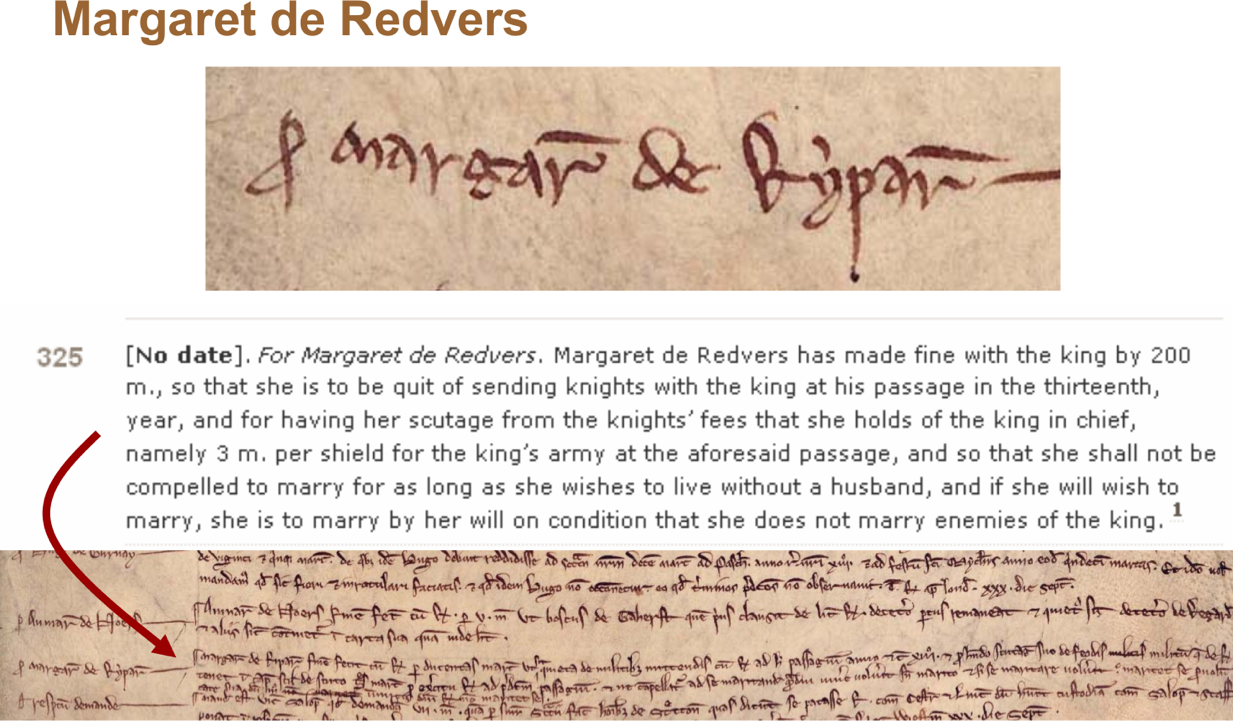
\includegraphics[width=\textwidth]{images/medieval_document}
	
\end{frame}


%%%%%%%%%%%%%%%%%%%%%%%%%%%%%%%%%%%%%%%%%%%%%


\begin{frame}
	\frametitle{Traces Through Time (3) -- Collaboration}
	
	\begin{itemize}
		\item The project set out as a collaboration between several institutes: \begin{itemize}
			\item The National Archives
			\item Institute of Historical Research
			\item Brighton University
			\item Leiden University
			\end{itemize}
		\item Brighton University worked on \emph{Natural Language Processing}.
		\item Our job was to perform record linkage on the extracted references delivered by Brighton University.
	\end{itemize}
	
\end{frame}


%%%%%%%%%%%%%%%%%%%%%%%%%%%%%%%%%%%%%%%%%%%%%

\begin{frame}
	\frametitle{Problem Definition (1)}
	
	\begin{block}{Record}
		A record $r$ is a tuple of $m$ attributes, each having a certain domain, that describes an entity, i.e., $r \in A_1 \times A2 \times \dots \times A_m$.
	\end{block}
	
	\begin{itemize}
	  	\item We assume that records are \alert{descriptions} of people.
	  	\item Records are potentially \alert{ambiguous}: they can describe more than one person.
	\end{itemize}
	
\end{frame}


%%%%%%%%%%%%%%%%%%%%%%%%%%%%%%%%%%%%%%%%%%%%%


\begin{frame}
	\frametitle{Problem Definition (2)}
	
	\begin{block}{Record Linkage}
		Given a set $\mathcal{R}$ of records, determine which of these records refer to the same entity.
	\end{block}
	
	\begin{itemize}
		\item Record linkage is a \alert{binary classification problem}.
		\item Record pairs are classified as \alert{matching} or \alert{non-matching}.
		\item The set of entities is usually unknown.
		\item Even with expert knowledge, it is hard to determine the match status of a record pair.
	\end{itemize}

\end{frame}


%%%%%%%%%%%%%%%%%%%%%%%%%%%%%%%%%%%%%%%%%%%%%


\begin{frame}
	\frametitle{Record Extraction}

	\begin{itemize}
		\item Instead of waiting for input from Brighton University, a simple context-free grammar was written in order to extract occurences.
  		\item First names and articles (of, de la, etc.) were used as anchor points in the text.
  		\item Capitalization, punctuation and ordering define the class of surrounding words.
  	\end{itemize}
  	
  	\begin{center}
  		\parsevar{first name} \parsevar{article} \parsevar{capitalized word} \\
  		$\downarrow$ \\ 
  		\parsevar{first name} \parsevar{article} \parsevar{last name}
  	\end{center}
\end{frame}


%%%%%%%%%%%%%%%%%%%%%%%%%%%%%%%%%%%%%%%%%%%%%


\begin{frame}
	\frametitle{Record Examples -- Fine Rolls of King Henry III}
	
	\begin{quote}
		\footnotesize
		``Concerning the corn of \underline{Roger of Hyde}. Order to the \underline{sheriff of Oxfordshire} to make the king’s advantage without delay, by the view of law-worthy men, from all of the corn of \underline{Roger of Hyde, knight}, in Hyde, who is with the Earl Marshal, and to put in gage etc. all those who he will find threshing that corn and intermeddling with the land of the same \underline{Roger} without warrant, to be before the king at his command to answer for it.''\footnotemark
	\end{quote}
	
	\begin{table}
		\footnotesize
		\centering
		\begin{tabular}{l l l l l}
	\toprule
	\textbf{Title} & \textbf{First name} & \textbf{Article} & \textbf{Last name} & \textbf{Role} \\
	\midrule
	& Roger & of & Hyde        & \\
	sherrif &       & of & Oxfordshire & \\
	& Roger & of & Hyde        & knight \\
	& Roger &    &             & \\
	\bottomrule
\end{tabular}
		%\caption{A possible segmentation of the paragraph taken from \emph{Fine Roll C 60/33}.}
		%\label{tab:segmentation}
	\end{table}
	
	\footcitetext{FineRolls}
	
\end{frame}


%%%%%%%%%%%%%%%%%%%%%%%%%%%%%%%%%%%%%%%%%%%%%


\begin{frame}
	\frametitle{Record Field Comparison (1)}
	
	\begin{itemize}
		\item Records are compared on a \alert{per-field basis}.
		\item Fields can be of many different types, but we assume \alert{strings}.
		\item Many different ways of computing distances between strings exist.
		\item To give an impression we will have a look at one particular approach.
	\end{itemize}
	
\end{frame}


%%%%%%%%%%%%%%%%%%%%%%%%%%%%%%%%%%%%%%%%%%%%%


\begin{frame}
	\frametitle{Record Field Comparison (2) -- $Q$-gram similarity}
	
	\begin{itemize}
		\item A $q$-gram is a sequence of $q$ characters.
		\item To compute the $q$-grams of a word, move a sliding window over the word.\begin{itemize}
				\item \framebox{Joh}n
				\item J\framebox{ohn}
			\end{itemize}
		\item String similarity between words defined as the similarity between their respective multisets of $q$-grams.\footnotemark
	\end{itemize}
	
	\pause
	
	\begin{equation*}
		\textrm{sim}_{\textrm{jaccard}}(\sigma_1, \sigma_2) = \frac{c_{\textrm{common}}}{c_1 + c_2 - c_{\textrm{common}}}
	\end{equation*}
	
	\onslide<1-2>\footcitetext{Ukkonen1992}

\end{frame}


%%%%%%%%%%%%%%%%%%%%%%%%%%%%%%%%%%%%%%%%%%%%%


\begin{frame}
	\frametitle{Record Field Comparison (3)}
	
	\begin{itemize}
		\item Many different string similarity functions exist. \begin{itemize}
			\item Edit distance\footnotemark: uses number of transformation steps.
			\item Soundex\footnotemark: phonetic similarity.
		\end{itemize}
		\item Similarity values can often be converted to distances, e.g., $\mathrm{dist}(\sigma)=1-\mathrm{sim}(\sigma)$.
		\item Distance function chosen depending on the content.
	\end{itemize}
	
	\footcitetext{Levenshtein1966}
	\footcitetext{Soundex}
	
\end{frame}


%%%%%%%%%%%%%%%%%%%%%%%%%%%%%%%%%%%%%%%%%%%%%


\begin{frame}
	\frametitle{Candidate Pair Classification (1) -- Distances}
	
	\begin{itemize}
		\item A distance function is defined for every field.
		\item The classifier first uses these functions to map a record pair to an array of distance values.
	\end{itemize}
	
	\vspace{-8mm}
	
	\begin{equation*}
		\mathrm{map}_{\mathrm{dist}}(\bm{r}_1, \bm{r}_2) \to (d_1, d_2, \ldots, d_n)	 \qquad \text{with } \left\vert \bm{r_1} \right\vert = \left\vert \bm{r_2} \right\vert = n
	\end{equation*}
	
	\pause
	
	\begin{itemize}
		\item Distance values are thresholded to obtain a binary value: fields are either \alert{equivalent} or \alert{nonequivalent}.
		\item If one or both values are missing, the fields are considered equivalent.
	\end{itemize}

\end{frame}


%%%%%%%%%%%%%%%%%%%%%%%%%%%%%%%%%%%%%%%%%%%%%


\begin{frame}
	\frametitle{Candidate Pair Classification (2) -- Probabilities}
	
	\begin{itemize}
		\item If a record field pair is equivalent, we look up the \alert{prior probability} of a person having that property, e.g., in a census.
		\item If such information is unavailable, we can compute the prior probability from the data.
		\item Equivalent, but are not unequal values, are treated as an \alert{equivalence class} and their probabilities are summed.
		\item Using the data itself introduces a bias towards `famous people', i.e., people that occur often.
	\end{itemize}

\end{frame}



%%%%%%%%%%%%%%%%%%%%%%%%%%%%%%%%%%%%%%%%%%%%%


\begin{frame}
	\frametitle{Candidate Pair Classification (3) -- Example}

	\begin{center}

        \begin{tabular}{| l | c | c | c |}
            \cline{2-4}
            \multicolumn{1}{l|}{ } & \textit{First name} & \textit{Article} & \textit{Last name} \\\hline
            $p$ & $0.182$ & $0.917$ & $0.00214$ \\\hline
            $r_1$ & John & de & Engelfield \\\hline
            \multicolumn{1}{c}{ } & \multicolumn{1}{c}{$0.0 \updownarrow$} & \multicolumn{1}{c}{ } & \multicolumn{1}{c}{$0.13 \updownarrow$} \\\hline
            $r_2$ & John & & Englefield \\\hline
            $p$ & $0.182$ &  & $0.00321$\\\hline
            \multicolumn{1}{l|}{ } & \textit{First name} & \textit{Article} & \textit{Last name}\\\cline{2-4}
        \end{tabular}
	        
	    \bigskip
	    
        \begin{tabular}{| l | c | c | c |}
            \cline{2-4}
            \multicolumn{1}{l|}{ } & \textit{First name} & \textit{Article} & \textit{Last name} \\\hline
            $p'$ & $0.182$ & & $0.0535$ \\\hline
            $E_q$ & $1$ & $1$ & $1$\\\hline
        \end{tabular}
       
     \end{center}
	
\end{frame}


%%%%%%%%%%%%%%%%%%%%%%%%%%%%%%%%%%%%%%%%%%%%%


\begin{frame}
	\frametitle{Candidate Pair Classification (4) -- Confidence}
	
	\begin{itemize}
		\item The last step of classification is to aggregate the probabilities in a \alert{confidence score}.
		\item Record pairs with nonequivalent fields are not considered for linking.
		\item Assume \alert{independence} of fields, e.g., \textit{First Name = John} does not affect the probability of \textit{Last Name = Williams}.
		\item The confidence score is computed as the sum of log probabilities:
	\end{itemize}
	
	\begin{equation*}
		\mathrm{conf}(\bm{p})=\sum_{i=0}^{\left\vert \bm{p} \right\vert}\log{p_i}
	\end{equation*}

\end{frame}


%%%%%%%%%%%%%%%%%%%%%%%%%%%%%%%%%%%%%%%%%%%%%


\begin{frame}
	\frametitle{Contextual Information (1)}
	
	\begin{itemize}
		\item The previously described procedure makes use of information that is relatively easy to obtain.
		\item Fields are often empty and the confidence score is therefore low.
		\item We may be able to exploit the fact that references occur within a certain \alert{context}.
	\end{itemize}

\end{frame}


%%%%%%%%%%%%%%%%%%%%%%%%%%%%%%%%%%%%%%%%%%%%%


\begin{frame}
	\frametitle{Contextual Information (2) -- An Example}

	\begin{quote}
	    ``A letter from the Secretary to Mr. Carkesse, desiring him to move the Commissioners of the Customs, that their Officers in the Out Ports may give this Board an Account of the quantities of Salt that is necessary and used in curing several species of Fish, was agreed and ordered to be sent.''
	\end{quote}
	
	\bigskip
	
	\begin{quote}
	    ``Ordered that Mr. Carkesse be desired to let this Board have on Tuesday next, if possible, the Account of Fish exported, which was desired the 17th of the last month.''
	\end{quote}
	
\end{frame}


%%%%%%%%%%%%%%%%%%%%%%%%%%%%%%%%%%%%%%%%%%%%%


\begin{frame}
	\frametitle{Contextual Information (3) -- Observations}

	\begin{itemize}
		\item Many \alert{stop words} occur that are probably not informative.
		\item There are a few interesting words: Customs, Fish, Salt.
		\item Individual words might be indicative of the \alert{topic} discussed.
		\item We need of means of extracting these words from the data.
		\item We propose \emph{Maximally k-Informative Itemsets}\footnotemark for this.
	\end{itemize}
	
	\footcitetext{Knobbe2006}
	
\end{frame}


%%%%%%%%%%%%%%%%%%%%%%%%%%%%%%%%%%%%%%%%%%%%%


\begin{frame}
	\frametitle{Maximally $k$-Informative Itemsets}
	
	\begin{block}{Joint entropy}
    	Suppose that $X = \left\{ x_{1}, \dots, x_{k} \right\}$ is an itemset, and $B = \left( b_{1}, \dots, b_{k} \right) \in \left\{ 0, 1 \right\}^{k}$ is a tuple of binary values. The \emph{joint entropy} of $X$ is defined as
    	\small
    	\begin{equation*}
        	H(X) = -\sum_{B \in \left\{ 0, 1 \right\}^{k}} p \left( x_{1} = b_{1}, \dots, x_{k} = b_{k} \right) \lg p \left( x_{1} = b_{1}, \dots, x_{k} = b_{k} \right)
    	\end{equation*}
    	\normalsize
	\end{block}
	
	\pause
	
	\begin{itemize}
		\item Presence and absence of items are treated equally.
		\item The maximum achievable entropy of an itemset of size $k$ is $k$.
	\end{itemize}

\end{frame}


%%%%%%%%%%%%%%%%%%%%%%%%%%%%%%%%%%%%%%%%%%%%%


\begin{frame}{Maximally $k$-Informative Itemsets}

	\begin{table}
	\centering
    \begin{minipage}{.3\textwidth}
        \centering
        \begin{tabular}{c c c c}
            \toprule
            $A$ & $B$ & $C$ & $D$ \\
            \midrule
            1 & 1 & 1 & 0 \\
            1 & 1 & 0 & 0 \\
            1 & 1 & 1 & 0 \\ 
            1 & 0 & 0 & 0 \\
            0 & 1 & 1 & 0 \\
            0 & 0 & 0 & 1 \\
            0 & 0 & 1 & 1 \\
            0 & 0 & 0 & 1 \\
            \bottomrule
        \end{tabular}
    \end{minipage}%
    \begin{minipage}{.3\textwidth}
        \centering
        \begin{tabular}{c c}
            \toprule
            $I$ & $H$ \\
            \midrule
            A & 1.00 \\
            B & 1.00 \\
            C & 1.00 \\
            D & 0.95 \\
            \bottomrule
        \end{tabular}
    \end{minipage}%
    \begin{minipage}{.3\textwidth}
        \centering
        \begin{tabular}{c c c}
            \toprule
            $I_{1}$ & $I_{2}$ & $H$ \\
            \midrule
            A & B & 1.81 \\
            A & C & 2.00 \\
            A & D & 1.41 \\
            B & B & 1.81 \\
            B & D & 1.41 \\
            C & D & 1.91 \\
            \bottomrule
        \end{tabular}
    \end{minipage}
\end{table}
	
\end{frame}


%%%%%%%%%%%%%%%%%%%%%%%%%%%%%%%%%%%%%%%%%%%%%


\begin{frame}{Maximally $k$-Informative Itemsets}

	\begin{block}{Maximally informative $k$-itemset}
	    Suppose that $I$ is a collection of $n$ items. An itemset $X \subseteq I$ of cardinality $k$ is a \emph{maximally informative k-itemset}, $\mathrm{iff}$ for all itemsets $Y \subseteq I$ of cardinality $k$,
	    \begin{equation*}
	        H(Y) \leq H(X)
	    \end{equation*}
	\end{block}
	
	\pause
	
	\begin{itemize}
		\item There are many itemsets that can be a Miki: $\dbinom{n}{k}$.
		\item Knobbe et al. proposed several algorithms for finding exact and approximate Mikis.
	\end{itemize}

\end{frame}


%%%%%%%%%%%%%%%%%%%%%%%%%%%%%%%%%%%%%%%%%%%%%


\begin{frame}{Maximally $k$-Informative Itemsets}

	\begin{center}
		\begin{algorithmic}[1]
	    \Function{ForwardSelection}{$k$, $n$}
	        \State $X:=\varnothing$
	        \For{$i:=1 \To k$}
	            \State $h_{\mathrm{max}}:=0$
	            \For{$j:=1 \To n$}
	                \State $h:=\textrm{JointEntropy}(X \cup \left\{j\right\})$
	                \If{$j \not\in X \textbf{ and } h \geq h_{\mathrm{max}}$}
	                    \State $h:=h_{\mathrm{max}}$
	                    \State $m:=j$
	                    \State $X:=X \cup \left\{m\right\}$
	                \EndIf
	            \EndFor
	        \EndFor
	        \State \Return $X$
	    \EndFunction
		\end{algorithmic}
	\end{center}
	
	\footcitetext{Knobbe2006}
	
\end{frame}


%%%%%%%%%%%%%%%%%%%%%%%%%%%%%%%%%%%%%%%%%%%%%


\begin{frame}{Maximally $k$-Informative Itemsets}

	\begin{itemize}
		\item Per definition, Mikis consist of items that are \alert{uncorrelated}.
		\item Roughly stated: items that occur frequently together are captured in the Miki by only one of the items.
		\item This makes the items within a Miki a good candidate for modelling `topics' of text segments.
		\item For each item in the Miki, we introduce a binary feature to the records, using the probability of each in the `lookup step` of the classifier.
	\end{itemize}
	
\end{frame}


%%%%%%%%%%%%%%%%%%%%%%%%%%%%%%%%%%%%%%%%%%%%%


\begin{frame}{Experiments -- Dataset}
	
	\begin{itemize}
		\item For validation of the system, we used manually annotated data from The Gascon Rolls project.
		\item The Gascon Rolls are records that were drawn up by the English royal administration of Aquitaine-Gascony (south-western France) between 1273 and 1468.
		\item Contain grants of land, oaths of treaties and other important documents.
		\item The dataset consists of so-called \emph{calendars}, which are summaries of the actual rolls.
	\end{itemize}
	
\end{frame}


%%%%%%%%%%%%%%%%%%%%%%%%%%%%%%%%%%%%%%%%%%%%%


\begin{frame}{Experiments -- Dataset}

\begin{table}
    \centering
    \caption{Overview of the size of the Gascon Rolls dataset.}
    \label{tab:data_overview}
    \begin{tabular}{l r}
        \toprule
        & Size \\
        \midrule
        Number of rolls & $66$ \\
        Number of membranes & $943$ \\
        Number of sections & $1153$ \\
        Number of occurrences & $30426$ \\
        Sum of file sizes & $27$ MB \\
        \bottomrule
    \end{tabular}
\end{table}
	
\end{frame}


%%%%%%%%%%%%%%%%%%%%%%%%%%%%%%%%%%%%%%%%%%%%%


\begin{frame}{Experiments -- Occurrence Extraction}

	\begin{itemize}
		\item The dataset contains $25 836$ 	annotated occurrences.
		\item A parser based on a context-free grammar was able to find and segment $22 206$ occurrences.
		\item Out of these $1684$ were not annotated and removed from the dataset resulting in $20 522$ segmented records.
		\end{itemize}

\end{frame}


%%%%%%%%%%%%%%%%%%%%%%%%%%%%%%%%%%%%%%%%%%%%%


\begin{frame}{Experiments -- Occurrences}

\begin{table}
	\footnotesize
    \centering
    \begin{tabular}{l l}
        \toprule
        \textbf{Field} & \textbf{Description}\\
        \midrule
        id & As provided in the source document.\\
        forename & \\
        article & Word(s) between the forename and surname.\\
        surname & \\
        provenance & Origin of a person.\\
        title & Used to address a person. \\
        role & Ascribed to person.\\
        regnal\_number & Used to distinguish monarchs.\\
        fileId & Filename \\
        sectionId & Section identifier. \\
        pos & Start position in section. \\
        endpos & End position in section. \\
        words & Words and their frequencies in section.\\
        orig & Original text.\\
        \bottomrule
    \end{tabular}
\end{table}

\end{frame}


%%%%%%%%%%%%%%%%%%%%%%%%%%%%%%%%%%%%%%%%%%%%%


\begin{frame}{Experiments -- Mikis}

	\begin{itemize}
		\item To reduce the number of items considered, several unpromising items were removed. \begin{enumerate}
    			\item \emph{Infrequent tokens}: any tokens that appear less than $5$ times are discarded.
    			\item \emph{Frequent tokens}: all tokens appearing in a fixed list of $319$ stop words were ignored.
    			\item Tokens that are part of \emph{occurrences}, such as first names, were ignored.
				\end{enumerate}	
	\end{itemize}
\end{frame}


%%%%%%%%%%%%%%%%%%%%%%%%%%%%%%%%%%%%%%%%%%%%%


\begin{frame}

	\onslide<1>{
		\begin{block}{Precision}
		    Precision, $E_{p}$, is the fraction of pairs that are correctly classified as true matches, i.e.,
		    \begin{equation*}
		        E_{p} = \frac{ \abs{\text{TP}} }{ \abs{\text{TP}} + \abs{\text{FP}} }
		    \end{equation*}
		\end{block}
	}
	
	\onslide<2>{
		\begin{block}{Recall}
		    Recall, $E_{r}$, is the fraction of true matches that are detected by the system, i.e.,
		    \begin{equation*}
		        E_{r} = \frac{ \abs{\text{TP}} }{ \abs{\text{TP}} + \abs{\text{FN}} }
		    \end{equation*}
		\end{block}
	}
	
\end{frame}


%%%%%%%%%%%%%%%%%%%%%%%%%%%%%%%%%%%%%%%%%%%%%


\begin{frame}

	\begin{block}{F-measure}
	    The general \emph{F-measure} measures the effectiveness of retrieval with respect to a user who attaches $\beta$ times as much importance to recall as precision in the following way:\footnotemark
	    \begin{equation*}
	        F_{\beta} = (1 + \beta^{2}) \cdot \frac{2 E_{p} E_{r}}{(\beta \cdot E_{p}) + E_{r}}
	    \end{equation*}
	\end{block}
	
	\begin{itemize}
		\item Details are not important: the F-measure is a means of combining precision and recall in one measure.	
	\end{itemize}

	\footcitetext{Rijsbergen1979}
	
\end{frame}


%%%%%%%%%%%%%%%%%%%%%%%%%%%%%%%%%%%%%%%%%%%%%


\begin{frame}

	\begin{table}
		\footnotesize
	    \centering
	    \pgfplotstabletypeset[%
    every head row/.style={before row=\toprule, 
    after row=\midrule},
    every last row/.style={after row=\bottomrule},
    col sep=semicolon,
    header=true,
    font=\small,
    columns/Word/.style={
        column type=l,
        string type
    },
    columns/Cum. Entr./.style={
        column type=c,
        fixed,
        fixed zerofill,
        precision=2
    },
    columns/p/.style={
        column type=c,
        fixed,
        fixed zerofill,
        precision=2
    }
]{tables/miki_words_gascon_short.dat}

	\end{table}

	%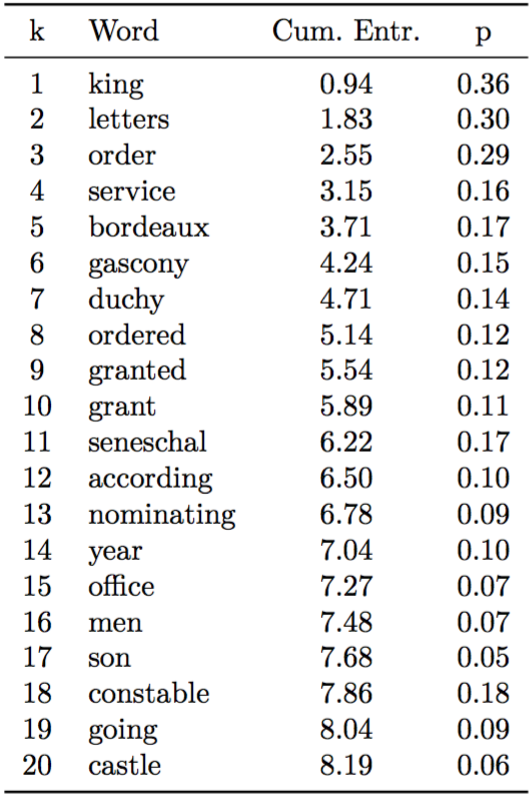
\includegraphics[width=\textwidth]{images/pic1}

\end{frame}


%%%%%%%%%%%%%%%%%%%%%%%%%%%%%%%%%%%%%%%%%%%%%


\begin{frame}[plain]

	\begin{figure}
	    \centering
	    \includegraphics[width=\textwidth,height=\textheight]{plots/miki_gascon.tikz}
	\end{figure}
	
	%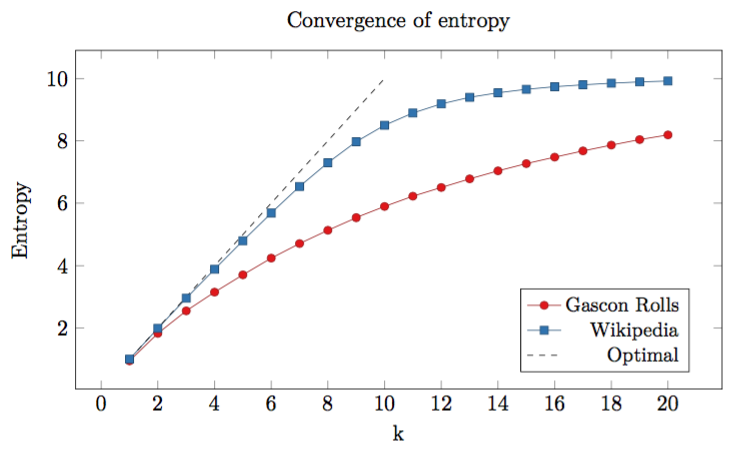
\includegraphics[width=\textwidth]{images/pic2}

\end{frame}


%%%%%%%%%%%%%%%%%%%%%%%%%%%%%%%%%%%%%%%%%%%%%


\begin{frame}[plain]
	\begin{figure}
	    \centering
	    \includegraphics[width=\textwidth,height=\textheight]{plots/kde.tikz}
	\end{figure}
	%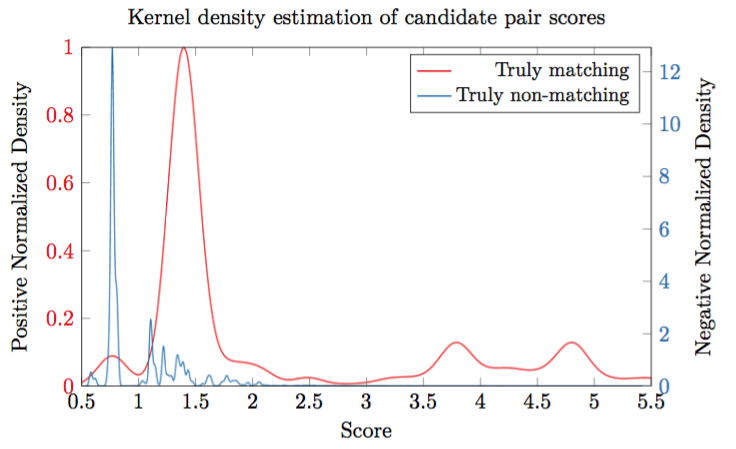
\includegraphics[width=\textwidth]{images/pic3}

\end{frame}


%%%%%%%%%%%%%%%%%%%%%%%%%%%%%%%%%%%%%%%%%%%%%


\begin{frame}[plain]
	\begin{figure}
    \centering
	    \includegraphics[width=\textwidth,height=\textheight]{plots/roc.tikz}
	\end{figure}
	%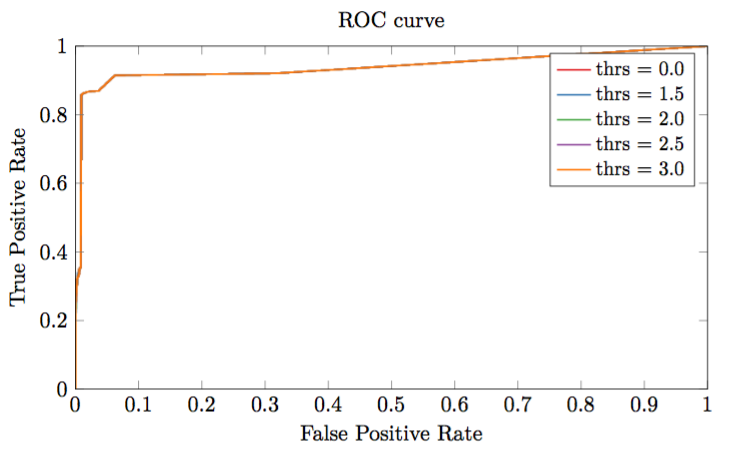
\includegraphics[width=\textwidth]{images/pic4}

\end{frame}


%%%%%%%%%%%%%%%%%%%%%%%%%%%%%%%%%%%%%%%%%%%%%


\begin{frame}[plain]
	\begin{figure}
    \centering
    \includegraphics[width=\textwidth,height=\textheight]{plots/precision_recall_curve.tikz}
	\end{figure}
	%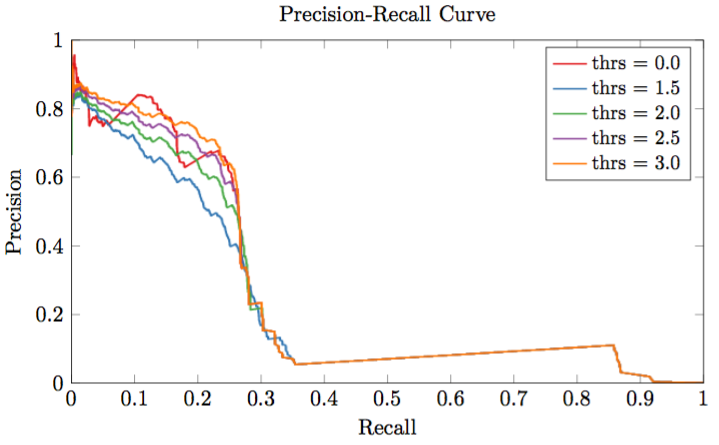
\includegraphics[width=\textwidth]{images/pic5}

\end{frame}


%%%%%%%%%%%%%%%%%%%%%%%%%%%%%%%%%%%%%%%%%%%%%


\begin{frame}[plain]
	\begin{figure}
	    \centering
	    \includegraphics[width=\textwidth,height=\textheight]{plots/f1.tikz}
	\end{figure}
\end{frame}


%%%%%%%%%%%%%%%%%%%%%%%%%%%%%%%%%%%%%%%%%%%%%


\begin{frame}{Conclusions (1) -- Occurrences}

	\begin{itemize}
		\item The grammar proved to do a reasonable job at extracting occurrences.
		\item Writing the grammar is a lot of work and dataset specific.
		\item Occurrence extraction was not the main focus of this project and should be done with more sophisticated methods.
	\end{itemize}

\end{frame}


%%%%%%%%%%%%%%%%%%%%%%%%%%%%%%%%%%%%%%%%%%%%%


\begin{frame}{Conclusions (2) -- Mikis}

	\begin{itemize}
		\item Mikis have not shown to have a significant impact on the performance of the record linker.
		\item There can be many reasons for this. \begin{enumerate}
 				\item Topic modelling does not give the kind of textual information we want.
 				\item Mikis are unable to model topics appropriately.
 				\item The usage of Mikis was incorrectly handled in the confidence score computation.
 			\end{enumerate}
 		\item More work is needed to be conclusive.
	\end{itemize}
	
\end{frame}


%%%%%%%%%%%%%%%%%%%%%%%%%%%%%%%%%%%%%%%%%%%%%

\begin{frame}{Conclusions (3) -- Record Linkage}

	\begin{itemize}
		\item The linker was able to retrieve about $30\%$ of the truly positive pairs with reasonable precision.
		\item The remaining part was hard to distinguish from the negative pairs, based on the confidence score.
		\item Candidate pairs are now compared in isolation.
		\item It might be worthwhile to research methods that consider pairs in a relational setting.
	\end{itemize}
	
\end{frame}


%%%%%%%%%%%%%%%%%%%%%%%%%%%%%%%%%%%%%%%%%%%%%


\begin{frame}

	\vspace*{\fill}
	
	\begin{center}
		\huge Fin
	\end{center}
	
	\vspace*{\fill}
	
\end{frame}



%%%%%%%%% TO-DOS %%%%%%%%%%

% Inleidend stuk over precision-recall, F1-measure
% Conclusie

% Bonus: plots netjes in LaTeX!

% Bonus bonus: zie hieronder.

% End slide with picture of thesis front page and URL to GitHub.

% Extra:
% Describe some of the benefits of studying the LaTeX source.
%     Data to be consumed by LaTeX in separate file (model-view approach)
%     Source syntax highlighting and formatting with minted.
%     Proper table formatting with booktabs
%     Doing all graphics with vectorized data formats to ensure a high-quality result.


\end{document}